% Kapitel 1

\section{Das Arduino Projekt}

Die Arbeit mit Mikrocontrollern und die Ansteuerung von Hardware hat selbst für Informatiker immer etwas Geheimnisvolles an sich – dafür müsse man wochenlang Datenblätter lesen und dann kryptischen Code schreiben, so die Vorstellung. Aber es geht auch anders! Jedenfalls seit 2005: Da waren es die Studierenden des Interaction Design Institute im italienischen Ivrea leid, mit ihren Computern nur über Tastatur und Maus zu kommunizieren. Sie suchten nach einer einfachen Möglichkeit, um ihre Ideen für neuartige Interaktionen zwischen Mensch und Maschine, ihre Kunst- und Roboterprojekte in funktionsfähige Prototypen umzusetzen. 

Massimo Banzi entwickelte daraufhin mit einer handvoll Mitstreitern ein einfaches, günstiges Mikrocontroller-Board samt Programmiersprache und Entwicklungswerkzeug und nannte es Arduino, nach einem lokalen König aus dem elften Jahrhundert.

Das kleine Entwicklungs-Board trat schnell einen Siegeszug an – gerade weil es sich nicht so sehr an lötende Nerds, sondern an Quereinsteiger wie Designer, Künstler oder auch Schüler richtete, die vorher nur in Ausnahmefällen Software entwickelt oder gar eigene Hardware gebaut hatten. 

\subsection{Was kann man mit dem Arduino alles machen?}

Das Netz ist voller Projekte, die von einer Laserharfe über twitternde Topfpflanzen bis zu autonom fliegenden Luftschiffen reichen.

Ich möchte das Projekt von Zoe Romano: 
\href{http://blog.arduino.cc/2014/07/17/a-low-cost-robotic-hand-tutorial-mirroring-your-own-fingers/}{A low-cost robotic hand (tutorial) mirroring your own fingers} (siehe Video)
genauer anschauen. Ziel dieses Projektes ist es die Bewegungen der Hand zu erfassen und auf eine RoboterHand zu übertragen.

Dieses Projekte besteht aus drei Teilen (siehe Abb. \ref{fig:sla}):
 
\begin{itemize}
  \item Einem Sensor, der Handschuh mit den Biegesensoren, die die Fingerbewegungen messen. 
  \item Einer Logik, das Arduino Board, das die Messwerte verarbeitet und die Bewegung steuert.
  \item Einem Aktor, der RoboterHand, die die Bewegungen ausführt. 
\end{itemize}
Diese Projekt ist ein gutes Beispiel für die Arbeitsweise eines Mikrocontrollers. Ein Mikrocontroller kann über Sensoren Daten einlesen  (Eingabe), diese Daten verarbeiten (Verarbeiten) und Aktoren (LEDs, Motoren, Lautsprecher, \dots) steuern (Ausgabe).   
\margininfo{Eingabe, Verarbeiten und Ausgabe: das EVA-Prinzip}

Genau wie dieses Projekt ist auch dieses Skript aufgebaut. Im ersten Kapitel erfährt du einiges über die Funktionsweise des Arduino-Boards. In Kapitel 2 wirst du mit verschiedenen Sensoren arbeiten und in Kapitel 3 wird schließlich die Funktionsweise verschiedener Aktoren thematisiert.
 
\begin{figure}[h]
\begin{center}
  \begin{tikzpicture}[remember picture]
    % Image 
    \node[anchor=south west,inner sep=0] (image) at (0,0) {\includegraphics[width=0.9\textwidth]{Kapitel1/Bilder/roboticHand}};
    % Marks 
    \draw[very thick, color=red,rounded corners=0.3cm] (0,1)  rectangle (3.5,7.5) node (sensor) at (1.75,1) {};
    \draw[very thick, color=red,rounded corners=0.3cm] (6,4)  rectangle (9,6.5) node (arduino) at (7.5,4) {};
    \draw[very thick, color=red,rounded corners=0.3cm] (13.5,0)  rectangle (17.5,7) node (actor) at (15.5,0) {};
    % comment
    \node[draw=red, fill=red!20, rounded corners,minimum width=0.2\textwidth, minimum height=1.4\baselineskip, anchor=west,align=center,text width=0.2\textwidth] (item1) at (0,-1) {Sensor: SenorHandschuh};
    \node[draw=red, fill=red!20, rounded corners,minimum width=0.2\textwidth, minimum height=1.4\baselineskip, anchor=west,align=center,text width=0.2\textwidth] (item2) at (6,-1){Logik: ArduinoBoard};
    \node[draw=red, fill=red!20, rounded corners,minimum width=0.2\textwidth, minimum height=1.4\baselineskip, anchor=west,align=center,text width=0.2\textwidth] (item3) at (13.5,-1){Aktor: RoboterHand};
    % grid 
  %\draw[color=red,help lines,xstep=1,ystep=1] (0,0) grid (18,8);
  %\draw[help lines,thin,xstep=.5,ystep=.5] (0,0) grid (18,8);
  %\foreach \x in {0,1,...,18} { \node [anchor=north] at (\x,0) {\x}; }
  %\foreach \y in {0,1,...,8} { \node [anchor=east] at (0,\y) {\y}; }  
  \path[red, thick,-] (sensor.south) edge [out=-90 , in=90] (item1);
  \path[red, thick,-] (arduino.east) edge [out=-90 , in=90] (item2);
  \path[red, thick,-] (actor.east) edge [out=-90 , in=90] (item3);
  \end{tikzpicture}
  \end{center}
  \caption{Aufbau eines Arduino-Projektes}
  \label{fig:sla}
\end{figure}

\subsection{Projekte und Ideen, die ohne Arduino wirklich schwer währen!}

Bevor du dich ausführlich mit dem Arduino Uno beschäftigst, möchte ich dir eine kurze Auswahl verschiedener Projekte vorstellen

\subsubsection{Manufaktur -- Arduino als Maker }

Werkstücke mit Hilfe eines PC fertigen, war bis vor kurzer Zeit nur mit sehr teuren CNC-Maschinen und teurer Spezialsoftware möglich.
\margininfo{CNC (Computerized Numerical Control) Computergestützte numerische Steuerung} 
Durch die Entwicklung des Arduino-Projekts (und anderer ähnlicher Projekte) wurde es möglich CNC-Maschinen und 3D-Drucker viel billiger zu bauen. Natürlich sind diese selbstgebauten Maschinen nicht mit industriellen Maschinen vergleichbar, dafür sind die aber um den Faktor 100-1000 billiger und somit in Bereichen einsatzbar die zuvor finanziell nicht möglich waren.
   
Zwei dieser Projekte möchte ich herausheben:
\begin{itemize}
  \item \href{http://www.shapeoko.com/}{Shapeoko An Open Hardware project by Edward Ford}
  \item \href{http://www.open-electronics.org/3drag-the-open-electronics-way-to-reprap/}{3Drag: the Open Electronics way to RepRap}
\end{itemize}
\begin{figure}[h]
  \begin{center}
    \subfigure[Shapeoko open hardware CNC-Fräse]{\includegraphics[width=0.5\textwidth]{Kapitel1/Bilder/Shapeoko.jpg}}
    \subfigure[3Drag open electronic 3D-Drucker]{\includegraphics[width=0.4\textwidth]{Kapitel1/Bilder/RepRap.jpg}}
    \label{fig:Manufaktur}
    \caption{Manufaktur: Arduino steuert CNC-Maschinen}
  \end{center}
\end{figure}


\subsection{Art und Design -- Arduino als Künstler}

Das Arduino-Board  wurde ursprünglich für die universitäre Ausbildung zum „Interaction Designer“ entwickelt. Die Motivation liegt darin Elektronik als kreatives Material einzusetzen. So kann mit Hilfe eines LED-Cubes (siehe Abb. \ref{fig:cube}) Musik als fallende Tropfen oder Silvesterraketen dargestellt werden. 

Mit einem Arduino LilyPad können intelligente Kleidungsstücke designed werden. Zum Beispiel eine Tasche, mit steuerbaren LEDs (siehe Abb. \ref{fig:bekathwia}).

\begin{itemize}
  \item \href{https://www.youtube.com/watch?v=6mXM-oGggrM}{LED cube 8x8x8 demo by chrmoe}
  \item \href{http://www.instructables.com/id/LilyPad-Arduino-Blinking-Bike-Safety-Patch/}{LilyPad Arduino Blinking Bike Safety Patch
by bekathwia}
\end{itemize}

\marginfigure{Kapitel1/Bilder/lillipad}{Arduino LilyPad}{fig:lillipad} 


\begin{figure}[h]
  \subfigure[LED Cube 8x8x8 by chr\label{fig:cube}]{\includegraphics[width=0.38\textwidth]{Kapitel1/Bilder/cube-7x7x7}}\qquad
  \subfigure[LilyPad Arduino Blinking Bike Safety Patch
by bekathwia  (by-nc-sa)\label{fig:bekathwia}]{\includegraphics[width=0.5\textwidth]{Kapitel1/Bilder/lillipad-proj}}
  \label{fig:Art}
  \caption{Art: Arduino als Künstler}
\end{figure}

%\subsection{Schuleprojekte mit dem Arduino}
%
%\begin{figure}[h]
%   \subfigure[Roboter Auto (Unterrichtsprojekt Klasse 9)]{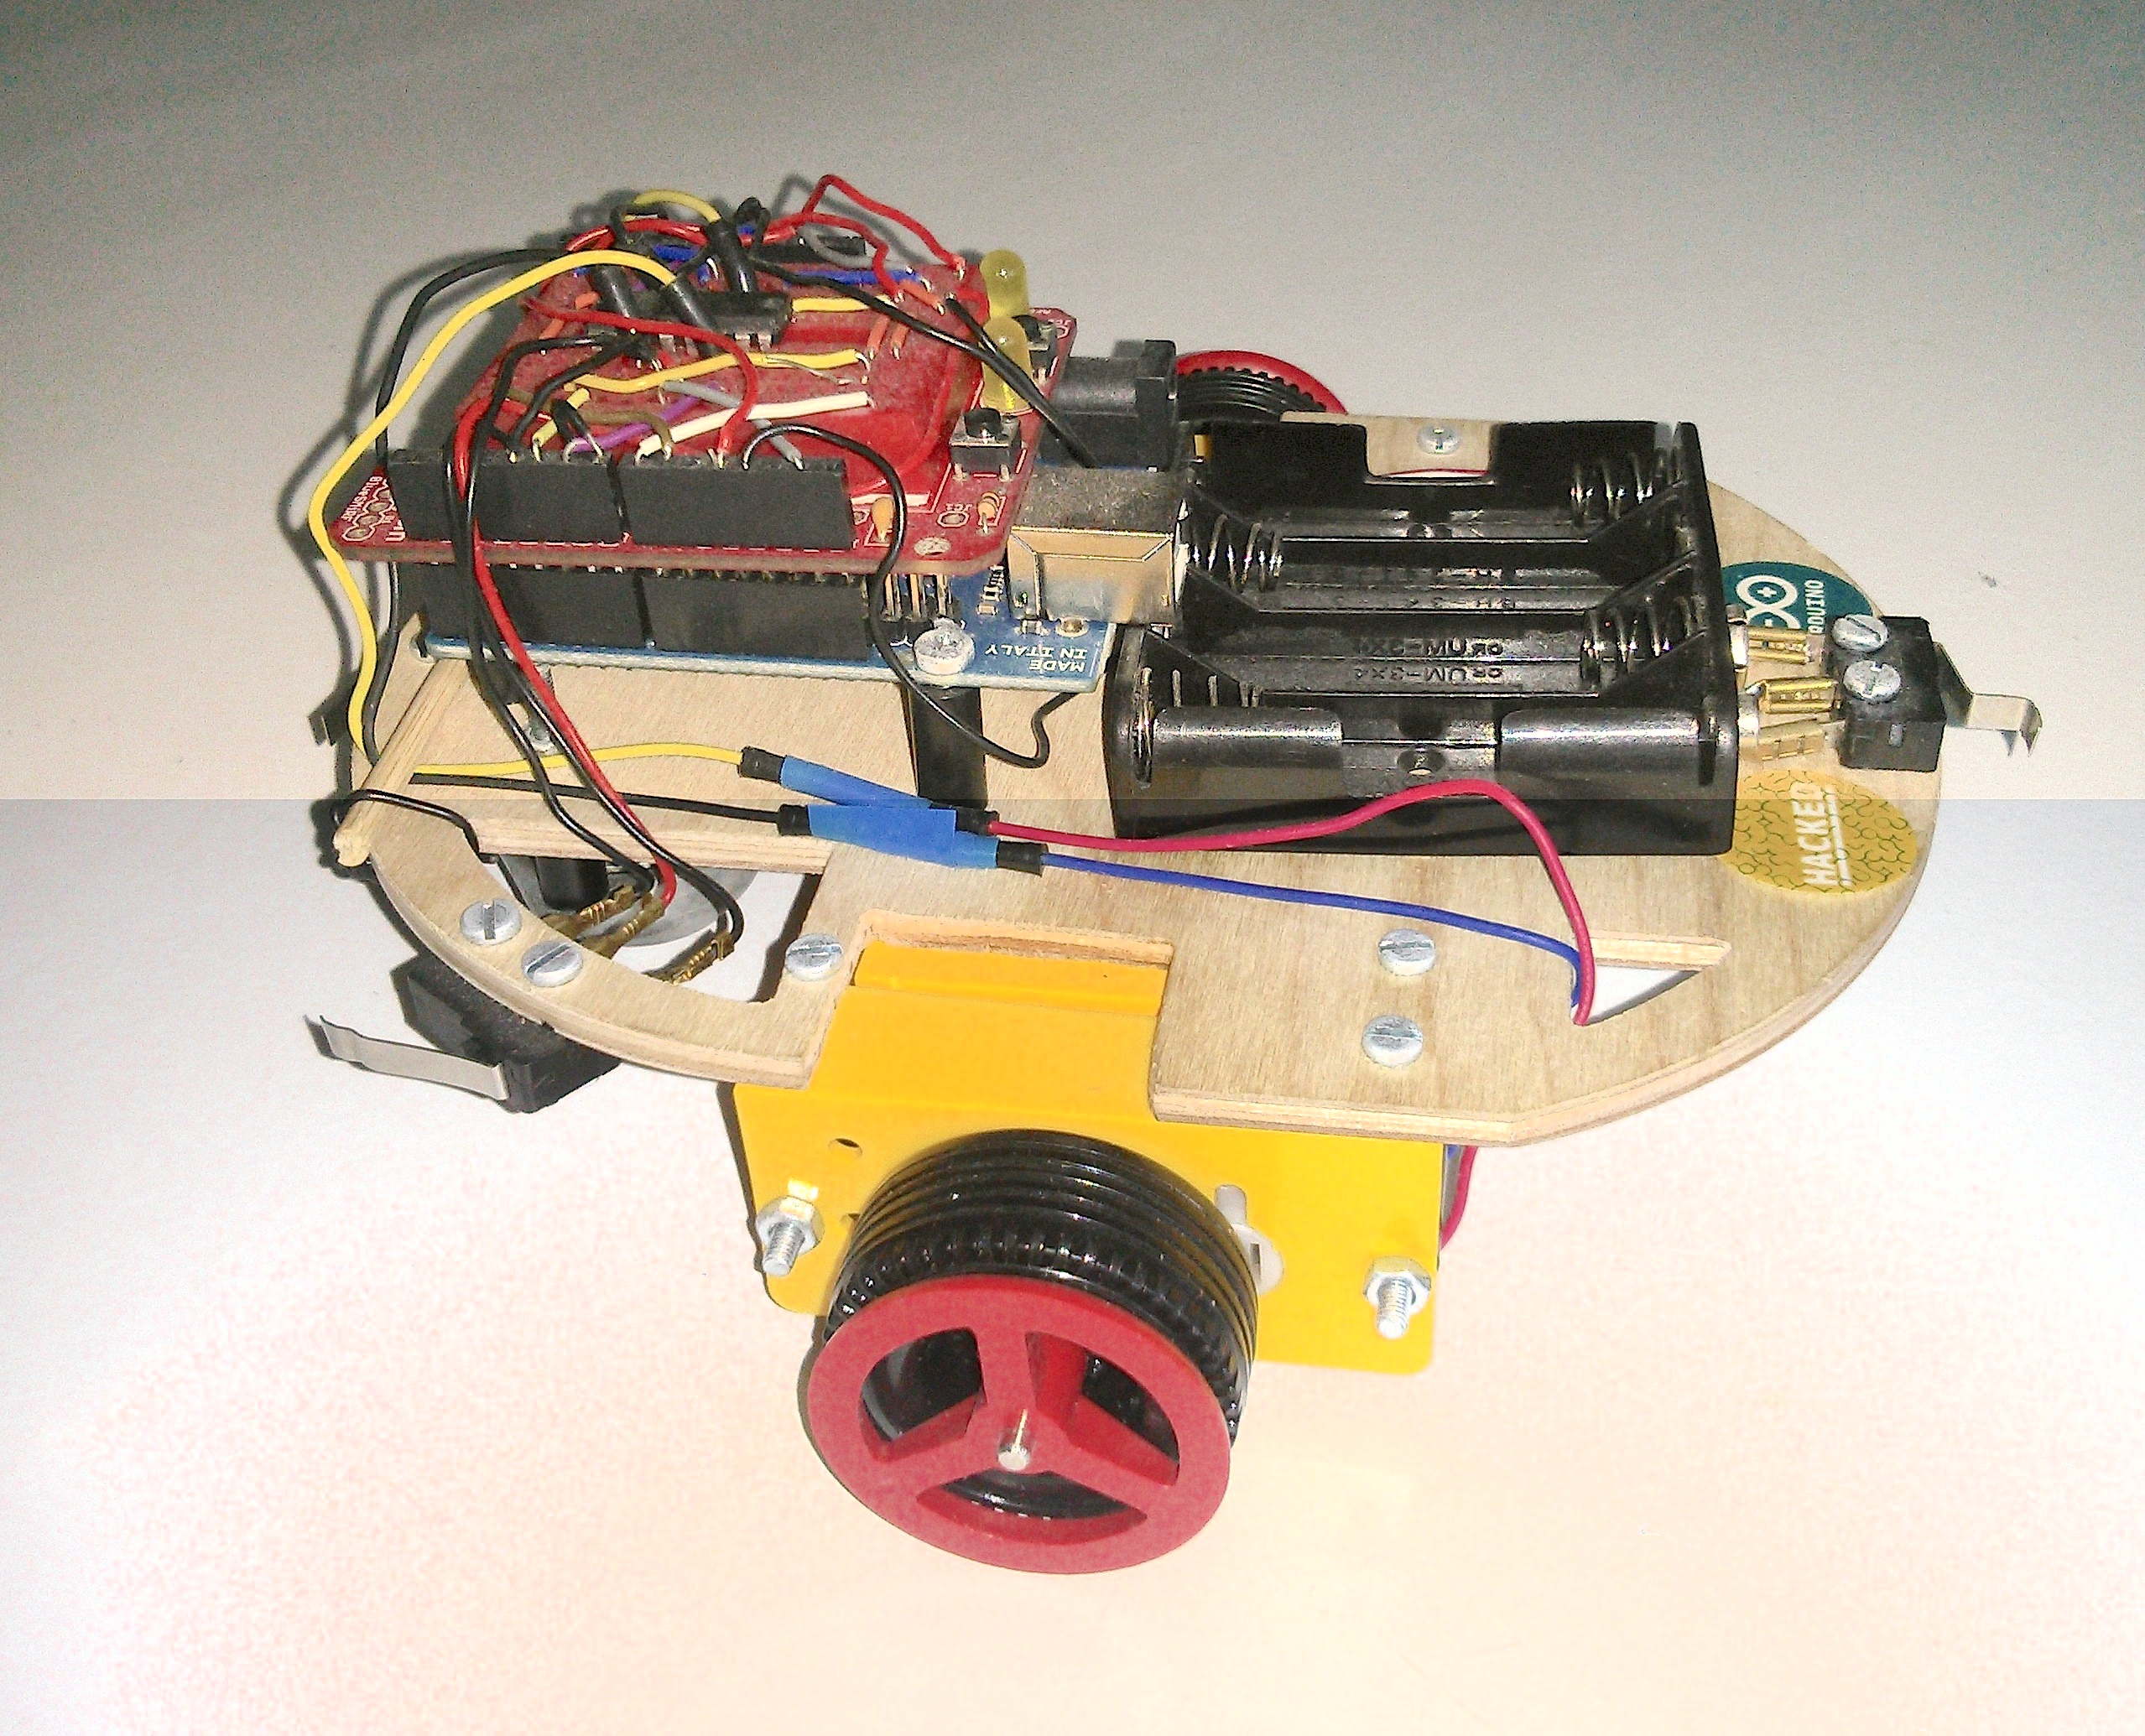
\includegraphics[width=0.35\textwidth]{Kapitel1/Bilder/robocar}}
%  \label{fig:Art}
%  \caption{Art: Arduino als Künstler}
%\end{figure}

\subsection{Der Mikrocontroller}

Der Kern eines Arduino ist der Mikrocontroller. Ein Mikrocontroller ist aus miniaturisierten elektrischen  Schaltkreisen -- den integrierten Schaltkreisen aufgebaut. 
\marginfigure{Kapitel1/Bilder/ATmega328}{Der ATmega328-Mikrocontroller (CC BY-NC-SA 3.0 by sparkfun.com)}{fig:ATmega328}

ICs sind komplexe elektrische Schaltungen, die auf kleinstem Raum in einem Siliziumkristall platz finden.
Was zu den Pionierzeiten der Elektronik noch mit unzähligen Bauteilen (Dioden, Transistoren, Widerständen und Kondensatoren) platzraubend Aufgebaut werden musste, findet heute auf kleinstem Raum platz in unterschiedlich großem schwarzen Plastikgehäusen mit einer bestimmten Anzahl von Beinchen, den sogenannten PINs. 
\margininfo{IC - Integrated Circuit} 

In der Abb. \ref{fig:ATmega328} siehst du den ATmega328-Mikrocontroller, der auch auf dem
Arduino Uno Board verbaut ist.  Du könntest ihn in dieser Form mit Hilfe einer geeigneten Spannungsversorgung und einem Taktgebers benutzten. Leider ist das aber sehr kompliziert. Aus diesem Grund wird der IC auf dem Arduino Uno Board montiert. Aufgabe dieses Entwicklungs-Boards ist es dir die Welt der Mikrocontroller auf möglichst einfache Weise zugänglich zu machen.

\subsubsection{Der innere Aufbau eines $\mu$Cs}

Der Aufbau eines Mikrocontrollers entspricht dessen eines Computers. Der Unterschied besetzt in der Leistungsfähigkeit, der Rechenleistung und im Speichervolumen.   

In der Abb. \ref{fig:blockdiagramm_yc} sind die Bestandteile eines ATmega schematisch dargestellt.

\marginfigure{Kapitel1/Tikz/blockdiagramm}{Blockdiagramm}{fig:blockdiagramm_yc} 

\begin{itemize}
  \item \textbf{Die CPU}  steuert und kontrolliert die anderen Teile des Mikrocontrollers durch dekodieren und ausführen von (Maschinen-)Befehlen. Sie kann den Speicher adressieren, Ein- bzw. Ausgänge verwalten und auf sogenannte Interrupts reagieren. 
  \item \textbf{Der Datenbus} verbindet alle Bestandteile des Mikrocontrollers miteinander. Die CPU fordert zum Beispiel Daten aus dem Speicher an, die Daten werden auf den Bus gelegt und können unmittelbar von der CPU verarbeitet werde.
  \item \textbf{Die Interrupt Steuerung (IRW)} kann auf  stattfindende Ereignisse reagieren. Dazu wird die aktuelle Aufgabe unterbrochen um sofort auf das Ereignis  reagieren zu können. 
  \item \textbf{Speicher RAM und ROM} (siehe Aufgabe)
\end{itemize}  

\subsection{Aufgabe:}

Was ist eigentlich der Unterschied zwischen RAM und ROM Speicher. Liese den Artikel \url{http://de.ccm.net/faq/3349-der-unterschied-zwischen-ram-und-rom} und erkläre die jeweilige Funktion ein eigenen Wörtern. 



\clearpage
\section{Das Arduino Uno Board}

Hier ist die neuste Version der Arduino-Hardware (Stand: März 2012) abgebildet, der Arduino 
Uno (R3)\index{Arduino Uno}. Die wichtigsten Anschlüsse und Bestandteile sind die folgenden:
\marginfigure{Kapitel1/Bilder/arduinouno}{Arduino Uno R3}{fig:arduinouno}
\begin{itemize}
\item[\textcolor{red}{A}] \textbf{Der Mikrocontroller} ist das wichtigste Bauteil des Arduinos. Beim Arduino Uno ist ein Atmel ATmega328 verbaut. 


\item[\textcolor{red}{B}] 
Über den \textbf{USB-Anschluss} verbindet man den Arduino mit dem PC. Über diese Verbindung überträgt man den Programmcode, das der Arduino ausführen soll, in den ROM Speicher des Mikrochips. Während das Programm ausgeführt wird, kann außerdem Daten zwischen PC und Arduino austauscht werden.

\item[\textcolor{red}{C}] 
Die rechte Buchsenleiste besteht aus 14 \textbf{digitalen Ein-} oder \textbf{Ausgängen}, sogenannten digitalen PINs. Ein digitaler PIN kann mit Hilfe eines Schalters oder Temperatur-Sensors Daten empfangen oder mit Hilfe eines Lautsprecher, einer Leuchtdiode oder einem anderem Bauteile Daten aussenden. Digital bedeutet, dass an den digitalen PINs entweder $0\V$ (digital 0/LOW) oder $5\V$ (digital 1/HIGH) Spannung anliegt. Ein digitaler PIN kann maximal 40mA Strom liefern.

Sechs digitale PINs besitzen noch die Zusatzfunktion der \textbf{PWM} (Pulsbreitenmodulation) \margininfo{PWM für pulse width modulation}. Diese PINs sind zusätzlich mit einer  \~  gekennzeichnet. 

\item[\textcolor{red}{D}] Der untere Teil der linken Buchsenleiste ist mit \textbf{Analog in} beschriftet. Mit Hilfe der analogen PINs können Spannungen zwischen 0V und 5V gemessen werden.

\item[\textcolor{red}{E}] 
die linke obere Buchsenleiste trägt die Bezeichnung \textbf{Power}:
   ``Vin'' (Voltage in) Eingangsspannung, ``Gnd'' (Ground)  0 Volt, ``5V'' (5 Volt), ``3V3'' (3,3 Volt), ``Reset''
\end{itemize}
Es gibt noch weitere Bauteile: Stromversorgung, Reset-Taster, Status-LEDs, Kondensatoren, Widerstände und einen Quarz.
 
\subsection{Aufgaben}

\subsubsection{Aufgabe 1:} 
Im PDF-File \href{http://marcusjenkins.com/wp-content/uploads/2014/06/ARDUINO_V2.pdf}{Arduino Uno V3 Pinout Diagram} ist der Aufbau des Arduino Uno nochmals sehr genau erklärt. Suche und kennzeichne alle GND-PINs, den Reset-Taster.    


\section{Software: die Arduino-IDE}

Die Arduino Entwicklungsumgebung\index{IDE} ist für Linux, OS X und Windows kostenlos verfügbar und kann von der Arduino Homepage heruntergelagen werden: \href{https://www.arduino.cc/en/Main/Software}{Download the Arduino Software}.

Die Entwicklungsumgebung besteht aus folgenden Teilen
\begin{itemize}
  \item[\textcolor{red}{A}]  den Menüs
  \item[\textcolor{red}{B}]  Texteditor zum schreiben des Programm-Codes
  \item[\textcolor{red}{C}]  einer Nachrichtenkonsole
\end{itemize}

Die Entwicklungsumgebung stellt automatisch eine Verbindung zur Arduino Hardware her um Programme hochzuladen und um weiter Daten mit dem Arduino auszutauschen. Ein fertiges Programme  wird ``Sketch'' genannt. Ein ``Sketch'' wird mit einem Text-Editor geschrieben und automatisch mit der Dateiendung ``.ino'' gespeichert. Jeder Sketch wird automatische in einem Eigenen Ordner gespeichert. Der Nachrichtenbereich gibt Feedback beim Speichern und Exportieren von Sketchen und eventuell auftretenden  Fehlern. 

\marginfigure{Kapitel1/Bilder/ide}{Die Arduino IDE (Version 1.0)}{fig:ide}

Die Bedeutung der Icons in der Symbolleiste \textcolor{red}{A} sind:
\begin{itemize}
  \item[] \includegraphics[width=0.03\textwidth]{Kapitel1/Bilder/verify} \textbf{Verify}:  Überprüft deinen Code auf syntaktische Fehler.
  \item[]  \includegraphics[width=0.03\textwidth]{Kapitel1/Bilder/play} \textbf{Play}: Kompiliert deinen Programmcode und lädt ihn auf das Arduino Board.
  \item[] \includegraphics[width=0.03\textwidth]{Kapitel1/Bilder/new} \textbf{New}: Erschafft einen neuen ``sketch''.
  \item[]  \includegraphics[width=0.03\textwidth]{Kapitel1/Bilder/open}   \textbf{Open}: Öffnet ein Menu mit allen Sketchen, die auf dem PC (deine eigenen Sketche und Beispiel-Sketche) gespeichert sind. Durch anklicken kannst du einen Sketch öffnen.
  \item[] \includegraphics[width=0.03\textwidth]{Kapitel1/Bilder/save} \textbf{Save}: Speichert deinen ``sketch''.
  \item[] \includegraphics[width=0.03\textwidth]{Kapitel1/Bilder/serial_monitor} \textbf{Serial Monitor}: öffnet ein Konsole, die über die USB-Schnittstelle eine serielle Verbindung zum Arduino aufbaut. 
\end{itemize}

\subsection{Aufgaben}

Starte die Arduino IDE. Verbinde mit dem UBS-Kabel dein Arduino Uno Board mit dem PC. Schaue im Menu ``Werkzeuge - Port'' nach, ob dein Arduino verbunden ist. Wenn dein Arduino richtig verbunden ist, dann kannst du ebenfalls im Menu ``Werkzeuge'' den ``Serieller Plotter'' öffnen. Erkläre die Funktion des Serieller Plotter's.  


\section{Blink, dein erster Arduino Sketch}\label{sec:blink}

\subsubsection{Vorbemerkungen}
Im ersten Teil dieser Einführung wirst du eine Ampelanlage mit Auto- und Fußgängerampel aufbauen und programmieren. Die benötigte Schaltung und den Sketch wirst du in den folgenden Abschnitten Stück für Stück erarbeiten. Es ist deshalb wichtig, dass du die jeweiligen Schaltpläne möglichst genau aufbaust. So sparst du Zeit, da du deine Schaltung nicht umbauen musst. 

\begin{figure}[h]
  \begin{center}
  \subfigure[Schaltplan]{\includegraphics[width=0.45\textwidth]{Kapitel1/Bilder/ampelFertig}}
  \subfigure[Reale Schaltung]{\includegraphics[width=0.45\textwidth]{Kapitel1/Bilder/ampelFertigReal}}
  \label{fig:ample}
  \caption{Die fertige Ampel}
  \end{center}
\end{figure}
  
\clearpage

\subsubsection{Jetzt geht es los!}

Um deinen ersten Arduino Sketch auf den Arduino zu übertragen und auszuführen musst du folgende Schritte nacheinander ausführen:

\marginfigure{Kapitel1/Bilder/arduino_blink_2}{Öffnen eines Sketches}{fig:blink2}

\begin{itemize}
  \item[1.] Starte die Arduino IDE und öffne das Beispiel ``Blink'' (siehe Abb. \ref{fig:blink2}).
  \item[2.] Verbinde nun das Arduino-Board und deinen PC mit Hilfe des UBS-Kabels.
  \item[3.] Drücke in der Arduino-IDE das Icon \includegraphics[width=0.03\textwidth]{Kapitel1/Bilder/play} um den Sketch zu übersetzen, auf den Arduino zu übertragen und um das Arduino-Programm auszuführen.
\end{itemize}

Jetzt sollte die kleine LED mit der Beschriftung ``L'' periodisch blinken.

\subsection{Eine externe LED blinken lassen}

Es kann auch eine ``externe'' LED zum Leuchten gebracht werden. Am schnellsten geht das, wenn man die LED direkt auf dem Arduino-Board in den ditigalen  Anschluß PIN13 und den daneben liegenden Anschluß GND steckt (siehe Abb. \ref{fig:arduino_blink_schaltung}). Sollte die LED von PIN13 blinken aber die externe LED nicht so hast du die LED falsch herum angeschlossen. 

\marginfigure{Kapitel1/Bilder/LEDmitWiderstand}{LED und Vorwiderstand}{fig:LEDmitWiderstand}

\margininfo{Achtung verbinde nie eine LED mit dem PIN Vin. Je nach Versorgungspannung wird die LED explosionsartig zerstört!}

\begin{figure}[h]
  \begin{center}
    \subfigure[Schnelle Methode]{\includegraphics[width=0.3\textwidth]{Kapitel1/Bilder/arduino_blink_schaltung}
      \label{fig:arduino_blink_schaltung_schnell}}
    \subfigure[LED mit Vorwiderstand an PIN 10]{\includegraphics[width=0.3\textwidth]{Kapitel1/Bilder/ampelG}
      \label{fig:arduino_blink_schaltung_vorwiderstand}}
    \caption{Anschluss einer externen LED}
    \label{fig:arduino_blink_schaltung}
  \end{center}
\end{figure}


Die schnelle Methode sollte nur zum Testen verwendet werden, da die LED kaputt gehen kann. Deshalb sollte eine LED immer zusammen mit einem Vorwiderstand betrieben werden (siehe Abb. \ref{fig:arduino_blink_schaltung_vorwiderstand}). Die Funktion des Vorwiderstandes ist es, die maximale Leistungsaufnahme der LED zu begrenzen. Für eine normale LED ist ein Vorwiderstand von $R=220\Ohm$ ausreichend. Mehr Wissen zum Thema Elektronik findest du im Anhang \ref{ch:anhang_elektronik} Hintergrundwissen Elektronik.

\subsubsection{Farb-Code von Widerständen} 

Wenn du die Abbildung \ref{fig:LEDmitWiderstand} den Widerstand genauer ansiehst, dann erkennst du die vier farbigen Ringe, die ersten drei Ringe ergeben den Widerstandswert, der vierte Ring die Fertigungstoleranz an. Es gibt viele Internetseiten, auf denen du die Farbcodes nachschauen kannst. Mein persönlicher Favorit ist die Seite \url{http://resisto.rs}. 

\marginimage{Kapitel1/Bilder/resistor_rs}


\clearpage
\subsection{Ein kurzer Blick auf den Sketch-Code} 

Der Arduino wird in der Computersprache C programmiert. C ist zwar alt, aber immer noch eine der beliebten  Programmiersprachen.
Schau dir den Programm-Code des Sketches ``Blink'' (siehe Listing \ref{lst:blink}) einmal genauer an. 

\begin{multicols}{2}
\begin{arduinoCode}{Blink}{lst:blink}
/*  (*@ \label{lis:blink_beginkommentar} @*) 
  Blink
  Turns on an LED for one second, then off for one second, repeatedly. 
                       (*@ \tikzmark{comment} @*)
  This example code is in the public domain.
*/ (*@ \label{lis:blink_endkommentar} @*)

void setup() {       (*@ \tikzmark{setup} @*)       
  // initialize the digital pin as an output.
  // PIN 13 has an LED connected on most Arduino boards:
  pinMode(13, OUTPUT);   (*@ \tikzmark{pinMode} @*)   
}   (*@ \label{lis:blink_endsetup} @*)   

void loop() { (*@ \label{lis:blink_beginloop} @*)         
  digitalWrite(13, HIGH);   (*@ \tikzmark{ledHigh} @*)
  // set the LED on
  delay(1000);    // wait for a second
  digitalWrite(13, LOW);    (*@ \tikzmark{ledLow} @*)
  // set the LED off
  delay(1000);    // wait for a second
} (*@ \label{lis:blink_endloop} @*)      
\end{arduinoCode}

\vfill
\columnbreak

\null\vfill
\begin{itemize}
  \itemsep45pt
  \item[] \tikzmarkcomment{item1}{Kommentarbereich: Hier wird die Aufgabe, Funktionsweise und weiter wichtige Informationen dokumentiert.}
  \item[] \tikzmarkcomment{item2}{Die setup()-Methode wird nur einmal ausgeführt}
  \item[] \tikzmarkcomment{item3}{PIN13 wird als  OUTPUT definiert.}
  \item[] \tikzmarkcomment{item4}{Die loop()-Methode wird immer wieder ausgeführt. Dadurch wird die LED für eine Sekunde (1000ms) eingeschalten und ...}
  \item[] \tikzmarkcomment{item5}{... anschließend ausgeschaltet. Nach einer weiteren Sekunde wiederholt sich das EInschalten.}
\end{itemize}
\vfill \null

\begin{tikzpicture}[remember picture,overlay]
  \path[red, thick,-] (comment.east) edge [out=0 , in=180] (item1);
  \path[red, thick,-] (setup.east) edge [out=0 , in=180] (item2);
  \path[red, thick,-] (pinMode.east) edge [out=0 , in=180] (item3);
  \path[red, thick,-] (ledHigh.east) edge [out=0 , in=180] (item4);
  \path[red, thick,-] (ledLow.east) edge [out=0 , in=180] (item5);
\end{tikzpicture}

\end{multicols}





\subsection{Die bisher verwendeten C Befehle}

In dem Sketch ``Blink'' werden unterschiedliche Strukturen der Programmiersprache C verwendet. Auf der Arduino Homepage
findest du unter \ArduinoHomepage{en/Reference/HomePage} alle C Sprachelemente, die du für die Programmierung eines Arduino nötig sind.

\margininfo{C wurde vom Informatiker Dennis Ritchie in den frühen 1970er Jahren an den Bell Laboratories für die Systemprogrammierung des Betriebssystems Unix entwickelte.}

Die Tabelle \ref{tab:blink_befehle} listet die bisher verwendeten Befehle auf und beschreibt kurz ihre Funktion. 
\begin{table}[h]
\begin{center}
  \tikzset{ 
    table/.style={
        matrix of nodes,
        row sep=-\pgflinewidth,
        column sep=-\pgflinewidth,
        nodes={
            rectangle,
            draw=black,text width=0.75\textwidth,
            align=center
        },
        minimum height=1.5em,
        text depth=0.5ex,
        text height=2ex,
        nodes in empty cells,
%%
        every even row/.style={
            nodes={fill=gray!20}
        },
        column 1/.style={
            nodes={text width=0.25\textwidth}
        },
        column 2/.style={
            nodes={text width=0.75\textwidth}
        },
        row 1/.style={
            nodes={
                fill=black!80,
                text=white,
                font=\bfseries
            }
        }
      }
  }
  \begin{tikzpicture}
  \matrix (first) [table,text width=6em]
  {   
 Name & Funktion \\
  \href{http://arduino.cc/en/Reference/PinMode}{pinMode(PIN, MODE)} & Konfiguriert den angegebenen PIN als 
 INPUT oder OUTPUT.  \\
 \href{http://arduino.cc/en/Reference/DigitalWrite}{digitalWrite(PIN, VALUE)} & Schreibt den VALUE mit einem Wert HIGH oder LOW auf den digitalen PIN.\\
 \href{http://arduino.cc/en/Reference/Delay}{delay(MS) } & Stoppt das Programm für MS Millisekunden. 1000ms entspricht einer Sekunde.\\};
\end{tikzpicture}
\end{center}
\caption{Übersicht der verwendeten C Befehle}
\label{tab:blink_befehle}
\end{table}%

\subsection{Aufgaben}

\subsubsection{Aufgabe 1}

\begin{description}
  \item[a)] Erstelle eine Tabelle, in der du alle C Sprache-Elemente und Strukturen dokumentierst. Orientiere dich an dem Aufbau der Tabelle  \ref{tab:blink_befehle}.   
  \item[b)] Lies auf \ArduinoHomepage{Reference/HomePage} die ausführliche englische Dokumentation der folgenden Befehlen
  \begin{enumerate}
    \item pinMode()  (\ArduinoHomepage{en/Reference/PinMode})
    \item digitalWrite()  (\ArduinoHomepage{en/Reference/DigitalWrite})
    \item delay()  (\ArduinoHomepage{en/Reference/delay})
  \end{enumerate} 
  Gibt es zusätzliche Informationen, die für dich wichtig sein können. Beantworte folgende Fragen schriftlich:
  \begin{itemize}
    \item Was passiert, wenn du einen digitalen PIN zum Steuern einer LED mit pinMode() auf INPUT setzt?
    \item Gibt es für digitale PIN noch weiter Modi?  
    \item Gibt es noch mehre delay()-artige Befehle? Eine Millisekunde ist zwar für einen Menschen eine unheimlich kurze Zeitspanne, für einen Arduino aber schon ziemlich lange!   
  \end{itemize}
  Ergänze deine Tabelle entsprechend.
  \item[c)]Verändere den Sketch ``Blink'' so, dass eine LED am PIN 10 SOS\footnote{Im Morse Alphabet: 
    3 mal kurz (für S) 3 mal lang (für `O') 3 mal kurz (für `S') gefolgt von einer langen Pause und dann wieder vor 
    vorne} blinkt. Den Schaltplan findest du in Abb. \ref{fig:arduino_blink_schaltung_vorwiderstand} 
    Speichere den veränderten Sketch unter dem Namen ``SOS'' ab.
  \item[d)] Erweitere deine Tabelle  mit der Befehlsübersicht um  den folgenden Befehl: 
  \begin{enumerate}
    \item random()  (\ArduinoHomepage{en/Reference/Random}).
  \end{enumerate}
  ein.
  \item[d)] Erstelle den neuen Sketch ``RandomBlink''. Die LED soll an PIN13 nun zufällig an- und ausgehen. 
  Dazu musst du in der loop()-Routine folgenden Befehl ergänzen ``delay(random(2000))''.  
\end{description}
\marginfigure{Kapitel1/Bilder/ampelGYR}{LEDs an PINs 10, 9 und 8}{fig:ampelGYR}

\subsubsection{Aufgabe 2: Steuern einer Autoampel}

Schließe an die digitalen PINs 10, 9 und 8 je eine grüne, gelbe und rote LED mit Vorwiderstand an. Die Schaltung findest du in Abb. \ref{fig:ampelGYR}. Erstelle den neuen Sketch `Ampel', der die 3 LEDs in der Lichtfolge einer Ampel leuchten lässt. Zuerst soll die gründe LED leuchten, achte dann auf die richtige Reihenfolge!


\section{Der Arduino Sketch}

Ein Arduino Sketch besteht aus mehreren  Bereichen:

\begin{itemize}
\item dem Kommentarbereich zur Dokumentation und Funktionsweise des Arduino Sketches. Ein ausführlicher Kommentarbereich hilft dir und anderen deinen Sketch zu verstehen. Du wirst oft auf deine selbst erstellten Sketche zurückgreifen.   
\item dem Definitionsbereich von Variablen 
  und Libraries
\item dem Mothodenbereich, mit der setup()-Methode, die einmal ausgeführt wird und der loop()-Methode, die immer wieder ausgeführt wird. Zusätzlich können noch weitere Methoden dazukommen (dazu aber später mehr). setup()- und loop()-Methode müssen in jedem Sketch vorhanden sein. 
\end{itemize}

\margininfo{Aus Platzgründen wir im folgendem der Kommentarbereich bei den Beispiel-Sketchen immer weggelassen. Du solltest aber bei jedem deiner Sketche einen ausführlichen Kommentarbereich schreiben.}
\begin{multicols}{2}
\begin{arduinoCode}{Bare Minimum}{lst:minimum}
/*        
  Sketch Name und Beschreibung 
  
  Datum:        (*@ \tikzmark{comment} @*) 
  Author:
  Version:
*/

// Definition von Variablen  (*@ \tikzmark{def} @*) 

void setup() {  (*@ \tikzmark{setup} @*)         
      
}

void loop() {   (*@ \tikzmark{loop} @*)         

}

\end{arduinoCode}

\vfill
\columnbreak

\null\vfill
\begin{itemize}
  \itemsep15pt
  \item[] \tikzmarkcomment{item1}{Kommentarbereich}
  \item[] \tikzmarkcomment{item2}{Definitionsbereich \\
  Z.B.: int ledPin = 13;}
  \item[] \tikzmarkcomment{item3}{setup()-Methode}
  \item[] \tikzmarkcomment{item4}{loop()-Methode}
\end{itemize}
\vfill \null

\begin{tikzpicture}[remember picture,overlay]
  \path[red, thick,-] (comment.east) edge [out=0 , in=180] (item1);
  \path[red, thick,-] (def.east) edge [out=0 , in=180] (item2);
  \path[red, thick,-] (setup.east) edge [out=0 , in=180] (item3);
  \path[red, thick,-] (loop.east) edge [out=0 , in=180] (item4);
\end{tikzpicture}

\end{multicols}



\subsection{Aufgaben}

\subsubsection{Aufgabe 1}
Dokumentiere die beiden Sketche ``SOS'' und ``Ampel''.

\section{Mit dem PC kommunizieren}\label{sec:kommunikation}

Bisher hast du, oder besser die ArduinoIDE mit dem Arduino ``gesprochen''. Jedes mal, wenn du einen Sketch auf das Board geladen hast. Natürlich kann man auch direkt mit dem Arduino sprechen. Dies geschieht über eine sogenannte Serielle Schnittstelle. Um zu verstehen wie das funktioniert, öffnest du den Beispielsketch ``DigitalReadSerial'' (siehe Abb. \ref{fig:digitalreadserial}).

\marginfigure{Kapitel1/Bilder/arduino_digitalreadserial}{``DigitalReadSerial'' öffnen}{fig:digitalreadserial}

Der Beispielsketch `DigitalReadSerial' ist in Listing \ref{lst:digitalreadserial} abgebildet. In der \textit{setup()}-Methode
wird zunächst eine serielle Verbindung zum PC hergestellt. Wichtig dabei ist die Übertragungrate von 9600 Baut/s.
Dann wird der digitale PIN2 auf INPUT gesetzt.   
\begin{multicols}{2}
\begin{arduinoCode}{digitalReadSerial}{lst:digitalreadserial}

void setup() {
  Serial.begin(9600); (*@ \tikzmark{serial} @*) 
  pinMode(2, INPUT);
}

void loop() {
  int sensorValue = digitalRead(2);
  Serial.println(sensorValue); (*@ \tikzmark{send} @*) 
}
\end{arduinoCode}
\vfill
\columnbreak

\null\vfill
\begin{itemize}
  \itemsep15pt
  \item[] \tikzmarkcomment{item1}{Serielle Kommunikation startet}
  \item[] \tikzmarkcomment{item2}{Aktuellen Sensor-Wert übermitteln}
\end{itemize}
\vfill \null

\begin{tikzpicture}[remember picture,overlay]
  \path[red, thick,-] (serial.east) edge [out=0 , in=180] (item1);
  \path[red, thick,-] (send.east) edge [out=0 , in=180] (item2);
 \end{tikzpicture}
\end{multicols}

Damit der Arduino etwas an den PC übermitteln kann, brauchst du noch einen Taster (eng. Button) mit dessen Hilfe du zwischen LOW und HIGH umschalten kannst.

\subsection{Aufbau der Schaltung}
Für die Schaltung brauchst du einen Taster und einen $10\kOhm$ Widerstand. 
\begin{figure}[h]
\begin{center}

\subfigure[Grundschaltung \label{fig:digitalreadserial_schaltung2}]{\includegraphics[height=0.4\textheight]{Kapitel1/Bilder/digitalreadserial2}}\qquad
\subfigure[Autoampel mit PushButton \label{fig:ampelButton}]{\includegraphics[height=0.4\textheight]{Kapitel1/Bilder/ampelButton}}
\caption{Das Schaltbild zum Beispiel Sketch ``DigitalReadSerial''}
\label{fig:digitalreadserial_schaltung}
\end{center}
\end{figure}



\subsection{Aufgaben}

\marginimage{Kapitel1/Bilder/10kOhm-button}

Erweitere deine Schaltung entsprechend Abb. \ref{fig:ampelButton}. Aus Platzgründen ist der PushButton näher an die rote LED eingebaut. Rechts wird der Platz noch gebraucht!
 
\subsubsection*{Aufgabe 1}

Testet die Schaltung zunächst mit dem Sketch ``DigitalReadSerial'' (siehe Listing \ref{lst:digitalreadserial}). Öffne den  ``Serieller Monitor'' im Menu ``Werkzeuge'' der Arduino LED. Schau dir die Ausgabe im ``Serieller Monitor'' an.

\subsubsection*{Aufgabe 2:}

Lies die Dokumentation zum DigitalReadSerial auf der Seite \ArduinoHomepage{en/Tutorial/DigitalReadSerial} genau durch und dokumentiere die folgenden Befehlen
  \begin{enumerate}
    \item Serial.begin()  (\ArduinoHomepage{en/Reference/Serial/Begin})
    \item Serial.println()  (\ArduinoHomepage{en/Reference/Serial/Println})
  \end{enumerate}
  
\subsubsection*{Aufgabe 3:}

Öffne dann den Sketch ``Button''  aus Beispiel/Digital. Schau die den Sketch genau an. Ergänze die Befehle (die noch nicht in deiner Tabelle dokumentiert sind) in deiner Tabelle. Schreibe den Sketch so um, dass die grüne LED verwendet wird.
\marginfigure{Kapitel1/Bilder/ampelFertig}{Push-Buttom mit LED}{fig:ampelButton}

\subsubsection*{Aufgabe 4: Projekt}

Erweitere deine Schaltung aus Aufgabe 3 entsprechend Abb. \ref{fig:ampelButton}, so dass du eine Autoampel (rot, gelb und grün) mit Fußgängerampel (rot und grün) mit Push-Button aufgebaut hast. Wenn ein Fußgänger auf den Kopf drückt (gedrückt hält), soll die Autoampel von grün auf rot schalten und die Fußgängerampel grün werden. Nach einer gewissen Zeit, soll die Autoampel wieder auf grün schalten.

\margininfo{Der Button muss lange gedrückt werden, da der Sketch nur an einer Stelle den Wert des Buttons auslesen kann. Später lernst du, wie du den Arduino programmieren kannst, damit er zu jeder Zeit den Button auslesen kann.}

\begin{multicols}{2}
\null\vfill 
\begin{arduinoCode}{Fußgängerampel mit Push-Button}{lst:fussgaengerample}
         (*@ \tikzmark{if} @*)
 if (digitalRead(2)) {
    // Fussgaengerample soll von rot auf gruen schalten und nach vier Sekunden wieder auf rot
      
 }
 
\end{arduinoCode}
\vfill\null 
\columnbreak

\null\vfill
\begin{itemize}
  \itemsep15pt
  \item[] \tikzmarkcomment{item1}{Hier reagiert der Arduino auf das drücken des Push-Buttons}
\end{itemize}
\vfill \null

\begin{tikzpicture}[remember picture,overlay]
  \path[red, thick,-] (if.east) edge [out=+25 , in=180] (item1);
  
\end{tikzpicture}


\end{multicols}


\sectionInformatik{C Sprachelemente: Variablen}

Daten zu speichern und zu verarbeiten ist eine zentrale Aufgabe eines Mikrocontrollers oder Computers. Die Programmiersprache stellt für diesen Zweck extra Variablen bereit.   

Eine Variable kannst du dir wie eine Art Box vorstellen. In so einer Box kannst du Zahlen, Wörter oder andere Dinge ablegen und du kannst sie später wieder hervorholen, um mit ihnen zu arbeiten.  Zum Beispiel können Messdaten eines Sensors gespeichert oder/und der gespeicherte Wert für eine Berechnung oder Ausgabe ausgelesen und/oder übergeben werden.

In diesem Abschnitt lernst du, wie Variablen für unterschiedliche Aufgaben erzeugt und manipuliert werden können.

\subsection{Das Erzeugen von Variablen}

Bevor eine Variable im Sketch verwendet werden kann, muss die Variable deklariert werden, d.h. es muss eine Box erstellt werden. \margininfo{Das Erstellen einer Variablen wird deklarieren genannt.} Deklarieren einer Variablen bedeutet, dass im Mikrocontroller Speicherplatz für die Variable zur Verfügung gestellt wird. In diesem Speicherbereich wird der Typ, und gegebenenfalls schon ein Wert gespeichert. \margininfo{Das Zuweisen eines Wertes wird initialisieren  genannt.} Variablen müssen nicht gleich initialisiert (ein Wert zugewiesen) werden, wenn sie deklariert werden, aber es ist oft nützlich ihnen einen definierten Anfangswert zuzuweisen.

\begin{multicols}{2}
\null\vfill 
\begin{arduinoCode}{Deklaration und Initialisation}{lst:deklarationinitialisation}
 int inVar1; (*@ \tikzmark{dek} @*)
 inVar1 = 9; (*@ \tikzmark{ini} @*)
  
 int inVar2 = 0; (*@ \tikzmark{dek-ini} @*)
\end{arduinoCode}
\vfill\null 
\columnbreak

\null\vfill
\begin{itemize}
  \itemsep15pt
  \item[] \tikzmarkcomment{item1}{Deklaration einer Variablen \textbf{inVar1}}
  \item[] \tikzmarkcomment{item2}{Initialisation einer Variablen \textbf{inVar1}}

  \item[] \tikzmarkcomment{item3}{Deklaration und Initialisation der Variablen \textbf{inVar2}}
\end{itemize}
\vfill \null

\begin{tikzpicture}[remember picture,overlay]
  \path[red, thick,-] (dek.east) edge [out=0 , in=180] (item1);
  \path[red, thick,-] (ini.east) edge [out=0 , in=180] (item2);
  \path[red, thick,-] (dek-ini.east) edge [out=0 , in=180] (item3);
\end{tikzpicture}


\end{multicols}

\subsection{Sinnvolle Namensgebung für Variablen}

Es ist extrem wichtig sinnvolle Namen für Variablen zu vergeben, damit sind Namen gemeint, die sich nach Möglichkeit selbst erklären. Doener1, doener2 mag zwar sehr lustig sein, aber du hast in zwei Wochen keine Ahnung mehr was du damit speichern wolltest! Darüber hinaus stellen die Variablen Doener und doener zwei Unterschiedliche Boxen dar. C unterscheidet Groß- und Kleinschreibung! \margininfo{C ist case sensitiv, das bedeutet die Variablennamen name, Name, NAME und naMe bezeichnen verschiedene Variablen}

\subsubsection{Tipps für sinnvolle Namen von  Variablen:}
Wenn du folgende Tipps befolgst, dann wirst du weniger Probleme haben!
\begin{itemize}
  \item Benenne deine Variable nach dem Inhalt: Wenn der Messwert eines Temperatur-Senors gespeichert werden soll ist ein sinnvoller Name measTemp (eng. measure messen).
  \item Benutzte die camelCase-Notation, d.h. der erste Buchstabe eines Variablennamens wird immer klein geschrieben. Wenn die Variable aus mehreren Wörtern zusammengesetzt ist, wird jedes Wort mit einem großen Buchstaben angefangen. Bekanntes Beispiel dieser Notation sind die Namen von Apple-Produkten:  iPhone, iPad, iPod, iMac aber auch McDonalds.
  \item Es gibt verschieden Variable-Typen. Oft ist es sinnvoll dass der Type der Variablen im Namen ablesbar ist. Zum Beispiel eine Variable die nur ganze Zahlen enthält wäre intVar eine gute Wahl. 
  \item Verwende nie ä,ö,ü oder ß. Diese Buchstaben werden vom C und der ArduinoIDE nicht unterstützt. Sonderzeichen (!, ?, /, - \_, \# etc.)  gehen auch nicht, diese Zeichen sind für (Rechen-) Operationen in C reserviert.    
\end{itemize}
Du wirst viele Beispiel-Sketche kennenlernen, die nicht der camelCase-Notation folgen. Das muss man auch nicht! Es macht aber Sinn, bestimmte sinnvolle Regeln bei der Vergabe von Namen in Programmen und für Dateinamen zu befolgen. Da sonst (bei größeren Programmen und vielen Dateien) sehr viel Zeit für die Suche nach Fehlern oder der richtigen Datei verloren geht!  Deshalb ist es sinnvoll, die camelCase-Notation von Anfang an immer zu benutzen.

\marginimage{Kapitel1/Tikz/camelCase}    

\subsection{Boxen mit Inhalt füllen}

Wenn eine Variable deklariert ist, kann ihr während des Programmablaufes mit Hilfe des Zuweisungsoperators 
(``='' Einfaches Gleichheitszeichen) ein Wert zugewiesen werden. Das Gleichheitszeichen ``='' hat die Aufgabe den Inhalt rechts, in die links stehend Box zu legen. Das Gleichheitszeichen hat in C eine andere Bedeutung als in der Mathematik! Besser wäre die Verwendung eines Pfeils ``$<-$'', leider hat man sich für das ``='' Zeichen entschieden.    
\margininfo{Das Gleichheitszeichen ist in C ein Zuweisungsoperator!}
\clearpage

\begin{multicols}{2}
\null\vfill 
\begin{arduinoCode}{Verwenden von Variablen}{lst:verwendung}
 intVar = 7;  (*@ \tikzmark{setzen1} @*) 
 
 inputVariable2 = analogRead(A2); (*@ \tikzmark{setzen2} @*) 
\end{arduinoCode}
\vfill\null 
\columnbreak

\null\vfill
\begin{itemize}
  \itemsep25pt
  \item[] \tikzmarkcomment{item1}{Weist der Variablen intVar den Wert 7 zu.}
  \item[] \tikzmarkcomment{item2}{Weist der Variablen intVar2 den Wert des analogen PIN A2 zu.} 
\end{itemize}
\vfill \null

\begin{tikzpicture}[remember picture,overlay]
  \path[red, thick,-] (setzen1.east) edge [out=0 , in=180] (item1);
  \path[red, thick,-] (setzen2.east) edge [out=0 , in=180] (item2);
\end{tikzpicture}

\end{multicols}


Sobald eine Variable gesetzt wurde (ein Wert zugewiesen), kann mit ihrem Wert gearbeitet 
werden. Z.B. kann überprüft werden, dass bestimmte Bedingungen erfüllt sind, oder der Wert
kann auch direkt  verwendet werden. 

\subsection{Für jeden Inhalt die passende Box}

\begin{table}[h]

\begin{center}
\tikzset{ 
    table/.style={
        matrix of nodes,
        row sep=-\pgflinewidth,
        column sep=-\pgflinewidth,
        nodes={
            rectangle,
            draw=black,
            align=center
        },
        minimum height=1.5em,
        text depth=0.5ex,
        text height=2ex,
        nodes in empty cells,
%%
        every even row/.style={
            nodes={fill=gray!20}
        },
        column 1/.style={
            nodes={text width=0.15\textwidth}
        },
        column 2/.style={
            nodes={text width=0.2\textwidth}
        },
        column 3/.style={
            nodes={text width=0.65\textwidth}
        },
        row 1/.style={
            nodes={
                fill=black!80,
                text=white,
                font=\bfseries
            }
        }
    }
}

\begin{tikzpicture}
\matrix (first) [table,text width=6em]
{   
  Variablentyp & Bedeutung  & Beschreibung \\
  int & Integer & ganze Zahlen (-32.768 bis 32.767) \\
  long & ganze Zahlen & (-2 Milliarden bis 2 Milliarden)\\
  float & Fließkommazahl & gebrochene Zahlen \\
  char & Character & Alphanumerische Zeichen (Buchstaben, Zahlen, Sonderzeichen) \\
  array & Variablenfeld & mehrere Werte eines Variablentyps können gespeichert werden \\
  String & Zeichenkette & Array aus mehreren alphanumerischen Zeichen \\
};
 \end{tikzpicture}
\end{center}
\caption{Auswahl an verschiedenen Variablentypen}
\label{tab:varTyps}
\end{table}%

Die beiden Variablentypen array und String sind etwas komplizierter aufgebaut und werden deshalb hier noch näher besprochen: 

\subsubsection{Arrays}

Bei Arrays handelt es sich im Grunde nicht um einen eigenen Typ von Variablen, sondern um eine Gruppierung mehrerer Variablen eines Typs.
\begin{arduinoCode}{}{}
int meineWerte[5] = {10,12,32,46,50};
\end{arduinoCode}
Im Beispiel wird als erstes ein Array vom Typ int angelegt. Die 5 in eckigen Klammern hinter dem Namen der Variable bestimmt die Anzahl der Speicherplätze, die das Array bereit stellt. Man nennt die Anzahl der Speicherplätze auch die Länge des Arrays.

Im Programm kann man durch die Verwendung eines Index auf die Speicherplätze des Arrays zugreifen. Die erste Stelle im Array ist die Stelle 0: meineWerte[0], der Wert ist 10 usw.

\begin{multicols}{2}
\null\vfill   
\begin{arduinoCode}{}{}
analogWrite(ledPin, meineWerte[0]); (*@ \tikzmark{mW0} @*)
analogWrite(ledPin, meineWerte[1]); (*@ \tikzmark{mW1} @*)
...
analogWrite(ledPin, meineWerte[4]); (*@ \tikzmark{mW4} @*)
\end{arduinoCode}
\vfill\null 
\columnbreak

\null\vfill
\begin{itemize}
  \itemsep15pt
  \item[] \tikzmarkcomment{item1}{Erster Wert: 10}
  \item[] \tikzmarkcomment{item2}{Zweiter Wert: 12}
    \item[] \tikzmarkcomment{item3}{Letzter Wert: 50}
\end{itemize}
\vfill \null

\begin{tikzpicture}[remember picture,overlay]
  \path[red, thick,-] (mW0.east) edge [out=0 , in=180] (item1);
  \path[red, thick,-] (mW1.east) edge [out=0 , in=180] (item2);
  \path[red, thick,-] (mW4.east) edge [out=0 , in=180] (item3);
\end{tikzpicture}


\end{multicols}


\subsubsection{String}
Es gibt verschiedene Möglichkeiten Textstrings darzustellen. Man kann entweder den Datentyp String verwenden oder einen String aus einem Array von Daten des Types char erstellen.
 
\begin{arduinoCode}{}{}
  String str1 = "arduino";
  char str2[8] = {'a', 'r', 'd', 'u', 'i', 'n', 'o'};
  char str3[ ] = "arduino";
  char Str4[8] = "arduino";
\end{arduinoCode}
Alle erzeugten Textstrings haben denselben Inhalt.


\subsubsection{Aufgabe 1}
Es gibt weitere Variablen-Typen. Informiere dich auf der Arduino Homepage \ArduinoHomepage{en/Reference/HomePage} über folgende Typen: 
boolean, unsigned int, short, double. 
Notiere ihre Bedeutung, ihre Beschreibung analog zur Tabelle \ref{tab:varTyps}.

\subsubsection{Aufgabe 2 (Projekt)}
Wie dir vielleicht aufgefallen ist, steht auf der Arduino Homepage \ArduinoHomepage{en/Reference/HomePage}  zweimal der Begriff String. Einmal klein und einmal groß geschrieben (siehe Abb. \ref{fig:string}). Das ist kein Fehler, sondern es sind wirklich zwei unterschiedliche Dinge. 

\begin{itemize}
  \item[] \textbf{string} bezeichnet ein Array, bei dem in jedem Feld Daten des Typs char gespeichert sind. 
  \item[] \textbf{String}: wiederum ist ein Text-Objekt. Objekt bedeutet in diesem Zusammenhang, dass es spezielle Funktionen gibt, mit welchen die im Objekt gespeicherten Daten manipuliert werden können. Funktionen die zu einem Objekt gehören, werden Methoden genannt.
\end{itemize}

\marginfigure{Kapitel1/Bilder/String.png}{Aufzug Arduino Homepage}{fig:string}

Objekte sind in der Informatik extrem wichtig. Mit dieser Aufgabe hast du die Möglichkeit einen ersten Blick auf sie zu werfen.

Auf der Seite \ArduinoHomepage{en/Reference/StringObject} werden die speziellen Funktionen anhand von Beispielen erklärt. Arbeite die zwei Punkte durch. Lade dazu den jeweiligen Beispiel-Sketch auf deinen Arduino und versuche zu verstehen was passiert. Beschreibe schriftlich in kurzen Sätzen deine Beobachtungen.
\begin{itemize}
  \item \ArduinoHomepage{en/Tutorial/StringConstructors}
  \item \ArduinoHomepage{en/Tutorial/StringAdditionOperator}
\end{itemize}


\subsection{Geltungsbereich von Variablen}

Für eine Variable wird immer (ihrem Typ entsprechend) eine bestimmte Größe an Speicherplatz reserviert. Die Größe dieses Speicherplatzes bestimmt den Wertebereich der Variablen.

%In Abb. \ref{fig:geltungsbereich} ist der Geltungsbereich einer Variablen mit 3 Bit Speicherplatz als Zahlenkreis dargestellt. Mit 3 Bit können die Binärzahlen $000$, $001$, $010$, $011$, $100$, $101$, $110$ und $111$ dargestellt werden.  Diese Binärzahlen stellen die Dezimalzahlen von 0 bis 7 dar. Wird jetzt eine Bereichsüberschreitung, z.B. durch eine Addition verursacht, wird entsprechend im Zahlenkreis weitergegangen.  
%\margintikzfig{\begin{tikzpicture}
%\def \n {7}
%\def \radius {2cm}
%\def \margin {8} % margin in angles, depends on the radius
%
%\foreach \s in {0,...,\n}
%{
%  \node[draw, circle] at ({360/(\n+1) * (\s)}:\radius) {$\s$};
%  \draw[->, >=latex] ({360/(\n+1) * (\s)+\margin}:\radius) 
%    arc ({360/(\n+1) * (\s)+\margin}:{360/(\n+1) * (\s+1)-\margin}:\radius);
%}
%\end{tikzpicture}
%}{Geltungsbereich einer 3 Bit Variablen}{fig:geltungsbereich}


Bei einer integer Variable ist der Wertebereich alle ganzen Zahlen zwischen $-32768$ und $32767$. Wenn man nun versucht einen größeren Wert z.B. 32770 in einer integer Variablen zu speichern wird eine sogenannte Wertebereich-Überschreitung (oder Überlauf) erfolgen. Beim Arduino wird um den zu großen Wert zu speichern einfach zum negativen Bereich ``weitergegangen''. Das heißt es wird der Wert $-32765$ gespeichert.
\begin{multicols}{2}
\null\vfill    
\begin{arduinoCode}{Überlauf einer integer Variablen}{lst:geltungsbereich}
  gBer = -32768; 
  gBer = gBer - 1;  (*@ \tikzmark{neg} @*)
  
  gBer = 32767;
  gBer = gBer + 1;  (*@ \tikzmark{pos} @*)
  
\end{arduinoCode}
\vfill\null 
\columnbreak

\null\vfill
\begin{itemize}
  \itemsep15pt
  \item[] \tikzmarkcomment{item1}{Wert der Variable ist jetzt 32767}
  \item[] \tikzmarkcomment{item2}{Wert der Variable ist jetzt -32768}
\end{itemize}
\vfill \null

\begin{tikzpicture}[remember picture,overlay]
  \path[red, thick,-] (neg.east) edge [out=0 , in=180] (item1);
  \path[red, thick,-] (pos.east) edge [out=0 , in=180] (item2);
\end{tikzpicture}
\end{multicols}

\subsubsection{Aufgabe 3}
Verändere \textbf{nichts} an deiner Schaltung. Erstelle den Sketch ``Ueberlauf''. Die Aufgabe ist, den Überlauf  der integer Variablen \textbf{gBer} ververanschaulichen. Führe dazu die Operationen aus Listing \ref{lst:geltungsbereich} in die setup()-Methode ein und übermittle mit Hilfe des Befehls Serial.println(gBer) den aktuellen Wert der Variablen gBer.  

\begin{multicols}{2}  
\begin{arduinoCode}{Versuche zur Überlauf einer Variablen}{lst:versuch-geltungsbereich}
int gBer; 
  
void setup() {
  Serial.begin(9600);
          (*@ \tikzmark{op} @*)
  Serial.println(gBer); (*@ \tikzmark{ser} @*)
}

void loop() {  
}
\end{arduinoCode}
\vfill\null 
\columnbreak

\null\vfill
\begin{itemize}
  \itemsep15pt
  \item[] \tikzmarkcomment{item2}{Füge die einzelnen Operationen aus Listing \ref{lst:geltungsbereich} ein}
  \item[] \tikzmarkcomment{item3}{Gibt nach jeder Operation den aktuellen Wert der Variablen aus}
  

\end{itemize}
\vfill \null

\begin{tikzpicture}[remember picture,overlay]
  \path[red, thick,-] (op.east) edge [out=0 , in=180] (item2);
  \path[red, thick,-] (ser.east) edge [out=0 , in=180] (item3);
\end{tikzpicture}
\end{multicols}

Lade deinen fertigen Sketch auf das Arduino-Board und öffne die Serielle Verbindung zum Arduino-Board. Dokumentiere deine Ergebnisse.


